%! Author = Ian's PC
%! Date = 10/25/2023

% Preamble
\documentclass[11pt]{article}

% Packages
\usepackage{amsmath}
\usepackage{romannum}
\usepackage{graphics}
\usepackage{graphicx}

\title{Assignment 4 Writeup}
\author{Ian Chen}
\date{\today}

% Document
\begin{document}
    \maketitle


    \section{Short answer problems}

    \begin{enumerate}
        \item \textit{What is the relation between image classification and object detection?
        Please give two concrete examples on how they are related (e.g., one is applied to solve another)?}\newline
        Image classification is often a component within object detection methods, helping to classify objects
        within localized regions. For example, a window-based object detection method may use an image classifier for
        each windows to classify objects within the window. Another example is the Viola-Jones face detection
        algorithm, which uses window-based object detection to detect faces, where image classifiers can be used to
        efficiently classify faces within each window. We can run image classification on windows of an image to
        detect objects within the image.

        \item \textit{Please compare semantic segmentation, instance segmentation and object detection.
        Describe the similarities and differences.}\newline
        Semantic segmentation is a deep learning algorithm that associates a label or category with every pixel in an
        image.
        It is used to recognize a collection of pixels that form distinct categories.
        Instance segmentation identifies the object instance each pixel belongs to.
        Object detection is a computer vision technique for locating instances of objects in images or videos.
        Instance segmentation builds on concepts in semantic segmentation by identifying object instances, however,
        it's more involved than semantic segmentation because it requires identifying the boundaries of each object
        and the pixels that belong to each object instance of the same categories.
        Instance segmentation identifies the pixels associated with each object instance, while object detection just
        produces the bounding boxes.
        These are similar in that they all involve identifying features and objects within an image, but they differ in
        that semantic segmentation is used to identify categories of pixels, instance segmentation is used to
        differentiate regions of pixels with the same label into different objects, and object detection is used to
        bound instances of objects to rectangular windows.

        \item \textit{Describe at least two plausible neural network designs for the task of semantic segmentations.}\newline
        Fully convolutional networks (FCNs) are a type of neural network that is used for semantic segmentation. We
        use feature maps to distinguish between different objects in an image.
        U-net is a type of FCN, where that FCN uses the final extracted features to up-sample, while U-net uses
        something called a shortcut connection to do that.
        Both of these neural networks employ the use of the encoder-decoder model, where the encoder extracts features
        while down-sampling the image, and the decoder up-samples the features to reconstruct the image.

        \item \textit{What are the applications of generative models in solving core computer vision tasks.}\newline
        Image synthesis, Object Detection/Segmentation, Image De-Noising, Image Super-Resolution/Upscaling.

        \item \textit{Discuss the differences between convolution neural networks and deconvolution neural networks.}\newline
        CNNs are foundational for extracting features and down-sampling, while deconvolutional networks are
        important in tasks that require up-sampling and the reconstruction of higher-resolution information.
        These techniques are often combined to form more complex models capable of handling diverse tasks.
        CNN extracts hierarchical features from the input image, while deconvolutional networks reconstruct images
        into higher resolutions or up-sampled.
    \end{enumerate}


    \section{Image Classification}

    Our task is to perform image classification using the CIFAR-10 dataset, which consists of 50K training images and
    10K testing images. We will experiment with two categories of methods: non-parametric methods and parametric
    methods.
    Our goal is to understand the performance of each method on this dataset. Our specific aims are:
    \begin{itemize}
        \item \textit{Compare the performance between K-Nearest Neighbor classifier and Adaptive Boosting classifier;}
        \item \textit{Analyze the performance of these two methods when varying the size of the training set
        and the size of the testing set;}
        \item \textit{Perform cross-validation to study the hyper-parameters of each method;}
        \item \textit{Try different feature representations.}
    \end{itemize}

    \begin{itemize}
        \item \textbf{Comparison.} Please compare the performance of the K-nearest neighbor classifier and the
        Adaboosting classifier. Which classes does K-nearest neighbor do better and which classes does Adaboosting do
        better, and
        why? How about running time?\newline
        For K-Nearest Neighbor classifier, the accuracy is about 33\% for small values of K. Once K becomes too
        large, then too many different image classes would match the testing image. L1 norm had a slight advantage
        over L2 norm, and the following 2 figures are tested with 1000 samples with no dimensional reduction.\newline
        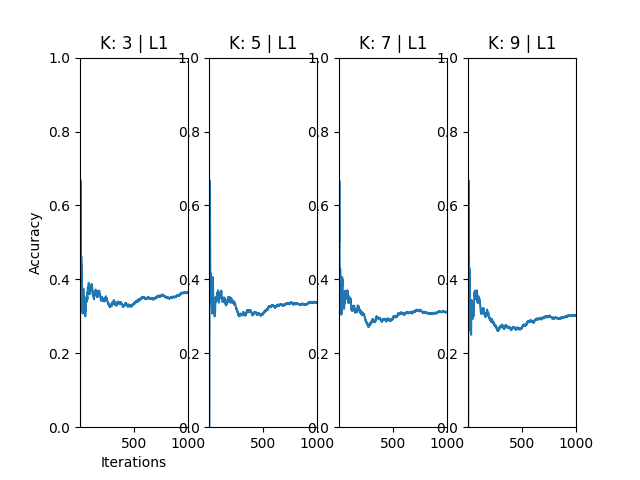
\includegraphics[width=\textwidth]{Output Pictures/Nearest Neighbors L1}
        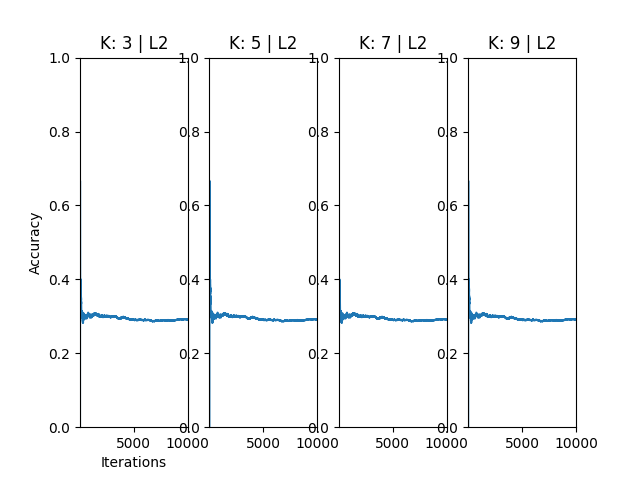
\includegraphics[width=\textwidth]{Output Pictures/Nearest Neighbors L2}
        For Adaptive Boosting classifier, the accuracy is about 11\%. This is because it's very biased towards the
        third label, the cat. The training time is very long, but the testing time is very fast.
        % TODO: Fix Adaboost accuracy
        K Nearest Neighbors has no training time, but since comparisons to the entire training set must be made for
        each test image, it has a very long testing time. This can be improved through PCA, where only
        certain components are considered for the nearest neighbor calculation. Adaboosting
        has a long training time, but since it only compares the binary strong classifiers instead of the entire
        training set to test each image, its running time to predict is much faster than K Nearest Neighbors.
        Additionally, I cached classifiers after training, so that each test wouldn't have to recompute the
        classifiers, but use the pre-trained ones. The ship class is one where KNN does better than Adaboosting, and
        the cat class is one where Adaboosting does better than KNN.

        \item \textbf{Cross-validation.} Perform 5-fold cross-validation for the K-nearest neighbor classifier.
        Report the optimized hyper-parameter K and the corresponding confusion matrix.\newline
        The optimal K for my KNN implementation was 1. I performed 5-fold cross-validation on the data set, and
        averaged about 37.2\% accuracy. The confusion matrix is shown below.\newline
        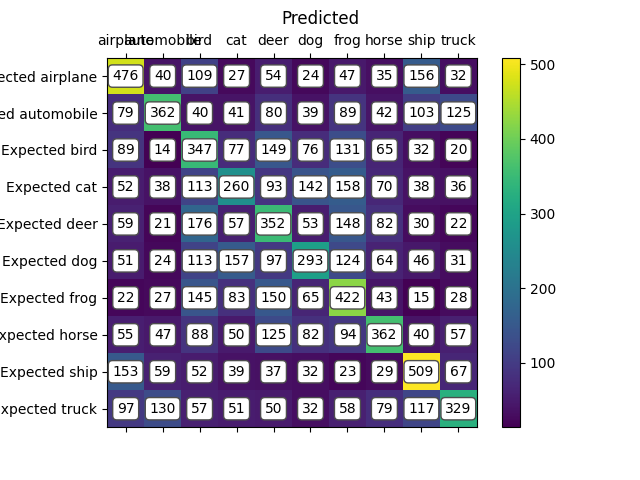
\includegraphics[width=\textwidth]{Output Pictures/Confusion Matrix KNN}

        \item \textbf{Cross-validation \Romannum{2}.} Perform 5-fold cross-validation for the AdaBoosting classifier.
        Report the optimal value for the number of weak classifiers.\newline
        The optimal number of weak classifiers for my Adaboosting implementation was 100. I performed 5-fold cross
        -validation on the data set, and averaged about 11.2\% accuracy. The confusion matrix is shown below.\newline
        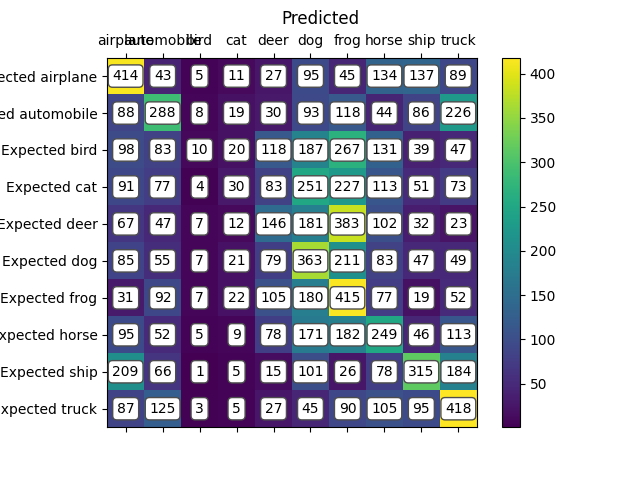
\includegraphics[width=\textwidth]{Output Pictures/Confusion Matrix AdaBoost}
        % TODO: Fix Adaboost accuracy
    \end{itemize}
\end{document}